
%\subsection{Сравнение}
\begin{frame}{Сравнение}
\begin{figure}
%Шахматные турниры...
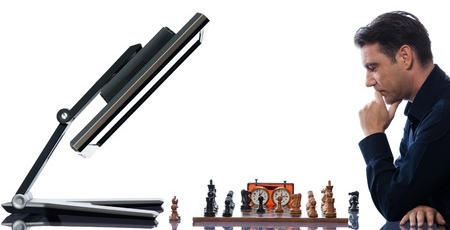
\includegraphics[scale=0.55]{./pictures/vs.png}
\end{figure}
\begin{columns}
\column{0.5\textwidth}
\begin{itemize}
\item Позиции анализируются независимо
\item Большой объем обрабатываемых данных
\item Сложно объяснить принципы выбора хода
\end{itemize}
\column{0.5\textwidth}
\begin{itemize}
\item Блочное восприятие
\item Ограниченный перебор
\item Прогрессивное углубление
\item Долгосрочное планирование
\end{itemize}
\end{columns}

%\smallskip
%Нет реализаций, учитывающих психологические аспекты.
\end{frame}

\begin{frame}{И всё-таки зачем?}
\begin{itemize}
\item Шахматы, как игра с полной информацией, сводится к решению задачи комбинаторной оптимизации.
\item Человек способен эффективно решать эту задачу не прибегая к полному перебору возможных вариантов.
\item Существующие игровые программы основываются на абсолютно иных методах решения.
\item Понимание принципов, которыми руководствется человек, может способствовать созданию эвристических алгоритмов решения других когнитивных задач.
\item Процесс мышления человека в настоящее время смоделировать не удалось.
\end{itemize}
\end{frame}

\begin{frame}{Что можно делать?}
Глобальная цель работы связана с попыткой решения следующих задач.
\begin{itemize}
\item Формальное описание модели, согласующейся с результатами психологических исследований мышления шахматистов.
\item Реализация алгоритма.
\item Проверка адекватности модели, например, путем сравнения траекторий движения глаз шахматистов и соответствующих элементов модели (цепочек, о которых будет рассказано далее).
\end{itemize}
\end{frame}

\endinput

\begin{frame}{Зачем этим нужно заниматься?} 
\begin{itemize}
\item Шахматы, как игра с полной информацией, сводится к решению задачи комбинаторной оптимизации.
\item Человек способен эффективно решать подобные задачи неформальным способом.
\item Существующие игровые программы основываются на иных методах решения.
\item В точности определить подход, используемый человеком, на данный момент не удалось.
\end{itemize}
\end{frame}


\begin{frame}{Сравнение и почему ничего не подходит}
\begin{itemize}
\item  практические результаты достигнутые программами значительно превосходят человеческие. Обыграли человека во всех играх (в т.ч. Го)
\item Анализ большого количества данных (статистических или в ходе построения дерева)
\item Не учитываются психологические аспекты.
\item Отсутствует стратегическое дальносрочное планирование.
\item Процесс мышления человека смоделировать не удалось.
\end{itemize}
\end{frame} 
